%% Matrix product state
%
% A matrix product state: arrays A on the chain, bonds between them, occupation
% indices n_i down -- a finite basis, so no wavy legs.
%
% Every tensor is a circle in the array colour. No tensor of this notation is
% a square: a square says nothing a circle does not, and on a lattice turned
% by 45 degrees it reads as a diamond. Shape carries meaning only where there
% is something to tell apart -- a triangle says isometric and a diamond says
% center (04, 05), a rounded box an operator on the chain.
%
% The fourth slot is the dots of a chain that goes on: the bonds either side of
% it stop at its border.
\documentclass[border=4pt]{standalone}
\usepackage{amsmath,amssymb}
\usepackage{tikz-tensors}
\input{notation}
\begin{document}
\begin{tikzpicture}
  \tnstack{P}{5}{ket}
  \tnlayer{P}{ket}{3*coef/$A$, dots, coef/$A$}
  \tnconnect{P}
  \tnopen[labels={$n_1$, $n_2$, $n_3$, $n_N$}]{down}{P}
  \tnmid{P-ket-1}{P-ket-2}{$D$}
\end{tikzpicture}
\end{document}
